% !Mode:: "TeX:UTF-8" 

\BiChapter{文本立场分析相关技术概述}{Methods of inserting figures}

\BiSection{引言}{Figures inserting standard from graduate school}
本章概要介绍立场分析及其相关技术。首先从目前研究相对成熟的文本情感分析入手,分别从传统的基于规则、机器学习、深度学习分别讨论文本情感分析技术。由于本文主要以深度学习的方法解决社交媒体中立场分析,所以详细分析深度学习在文本情感分析的研究。作为本文的重点研究对象详细介绍了分别基于机器学习和深度学习模型的文本立场分析技术相关研究 本章总结了各项研究工作的特点,在分析优缺点的基础上引出本文的后续研究



\BiSection{文本情感分析相关技术概述}{Captions and descriptions of figures}
文本情感分析,指用自然语言处理、文本挖掘以及计算机语言学等方法来识别和提取原素材中的主观信息。通常来说,情感分析的目的是为了找出说话者或作者在某些话题上或者针对一个文本两极的观点的态度。这个态度或许是他或她的个人判断或是评估,也许是他当时的情感状态,或是作者有意向的情感交流。文本的情感分析是自然语音处理的重要研究内容之一,且其具有重要的科研价值与商业实用价值,吸引了大量的研究人员的关注。研究人员从不同的角度和不同方法对文本情感分析展开了研究。本节将从基于情感词典、机器学习和深度学习的三个方向分别概述近年来情感分析的研究进展。


\BiSubsection{基于情感词典的文本情感分析相关技术}{Recommended figure format applied in \LaTeX}
基于情感词典的文本情感分析是早期研究人员的成果,其相应的模型建立在情感词典和语言学的规则基础上。由于模型的解释性好,需要计算资源较少,成为早期研究文本情感分析的主流。情感词典作为文本情感分析的重要组成部分能给文本情感分析提供重要的特征信息。情感词典的构造通常由语言学领域的专家完成。例如现有相对成熟的情感词典有WordNet、HowNet、大连理工大学中文情感词汇文本库等。基于情感词典的文本情感分析的技术步骤通常先匹配原文本中与情感词典相对应的情感表达特征词,然后根据各特征词的表达方式综合计算其每一个特征词的情感得分,最后结合整个文本的情感得分总结文本的情感倾向。

Taboada【】在原来情感词典的基础上进一步考虑了词语的词性,结合情感词和词性综合给出情感的倾向得分。该情感分析模型包含一个语义指向计算器(Semantic orientation calculator,so-cal),这个计算器首先抽取出文本中的形容词、动词、名词以及副词等情感方位词,然后结合各种情感方位词计算原来文本的情感指向,模型结合的情感指向和强调、弱化、否定等转移的价位得到文本最终的情感倾向。作者通过一系列的实验证明了基于情感词典和此种转移规则的模型具有很强的鲁棒性,在跨领域的的文本情感分析上也有良好的表现。孙建旺【】等提出结合情感词典和机器学习两者的优势来解决微博情感分析的问题利用微博多层次结构对微博文本进行特征降维。此外,由于微博包含多种颜文字,表情符等特点,设计了对颜文字和表情符的情感计算方法,其实验证明了加入表情符等特征,对微博的情感分析效果得到了提高。

基于不同的上下文可能决定某些情感词的特点,具有一定的领域相关性。例如“高”在“质量高”的上下文中表达的是正面的情感倾向,但是如果在“消费高”的上下文则表达负面的情感倾向。Bollegala【】等人结合了不同领域对情感词的表达特点构造了领域相关的情感词典。实验证明结合领域知识的情感词典能在相对于的领域取得更好的效果。Li【】提出一种相关领域自适应情感词的框架,能同步从标注训练语料中提取出的主题词和情感词,并进一步通过分析标注语料中主题词和情感词的关系来推导出未标注语料中与主题相关的情感词。

总体来看,基于情感词典/规则和知识库的情感分类准确率较高,但由于情感词典和常识库规模的限制,覆盖率较低。同时此类方法对分词、词性标注、规则匹配等的准确性要求较高,系统内部错误传递影响较大。[30]

\BiSubsection{基于机器学习的文本情感分析相关技术}{Recommended figure format applied in \LaTeX}

随着机器学习成功应用于其他领域的快速发展,对于文本情感分析的问题,大量的研究人员开始开展基于机器学习的文本情感分析的研究。基于机器学习的文本情感分析方法,首先通过特征工程抽取文本情感分析特征,然后通过抽取出来的特征词用机器学习能理解的数值表达文本。通过人工标注建立起特征表示数据和情感类标对的训练数据,通过各种已有的机器学习模型(支持向量机、朴素贝叶斯、逻辑回归、最大熵模型等)提取出训练集中特征和类标之间的映射关系的模型。Sida Wang【42】等利用N元词组(N-gram)对文本情感进行建模,模型结合了朴素贝叶斯与支持向量机的两个模型。首先利用朴素贝叶斯的思想,计算每一个词组的对数计数概率r,公式如下:


$$r=\log(\cfrac{\cfrac{p}{\|p_1\|}}{\cfrac{q}{\|q_1\|}})$$
$$p=\alpha + \sum_{i:y^{(i)}=1}f^{(i)}$$
$$p=\alpha + \sum_{i:y^{(i)}=-1}f^{(i)}$$
其中$y^{(i)}$为训练实例$i$的类标,$y^{(i)}\in\lbrace-1,1\rbrace$。其中$f^{(i)}$为训练实例$i$的特征向量,$f_{(i)}\in R^{\|V\|}$, $V$为特征集合 $\alpha$为平滑因子。

于上述r的计算公式可知,从训练语料中可以计算出每一个词语对于不同情感的倾向大小,所以利用我们已经计算的每一个词的r值,可以得到文本的特征表示,特征表示后的文本可以作为支持向量机的输入,通过支持向量机可以抽取出训练集中有关文本情感分析的模式。

Pang[8]等研究者创新性的把文本主题分析的技术迁移应用到文本情感分析中,文本的话题分类主要根据与话题相关的主题词决定,但是表达情感的方式更加的多样化,需要考虑的因素更多。Pang把文本的情感分析看成一类特殊的主题分析,使用了在有监督学习上泛化能力较好的支持向量机、朴素贝叶斯、最大熵模型三种基础的分类模型。选用的分类特征为一元词组(Unigram)、二元词组(Bigram)、词性分析(POS)、形容词位置信息等。此研究通过组合特征和模型的交叉验证表明,三个分类器组合任意一个特征的性能都比基线模型要好,在有关电影影评的数据集上,一元词组(Unigram)结合支持向量机的模型取得了良好的效果。但是此研究实验也论证了文本的情感分析的性能还是和文本主题分析存在较大的差距,同时也佐证了文本情感分析对模型和特征也有更高的要求。

为了减少文本中无关的客观信息对文本情绪分析的干扰作用,Pang和lee对上述基于机器学习的文本情感分析模型进行了有针对性的改进,规避了文本客观消息的干扰,使模型更加专注于文本的主观信息。作者他们把原来的文本情感分析问题转换成以各字句连接图中最小割问题,应用了挖掘图中的最小割的分类器来寻找对情感分析有用的主观表达的句子,从而屏蔽掉客观消息的干扰。此研究的实验也论证了剔除客观信息的文本情感分析模型的性能得到显著的加强。

\BiSubsection{基于深度学习的文本情感分析相关技术}{Recommended figure format applied in \LaTeX}

深度学习由于其更复杂的模型和更多的参数,比起以往的的机器学习方法在海量数据集上更有优势。且深度学习具有能够以端到端的形式构建模型的优势,不再需要人工筛选和总结大量特征,所以得到了情感分析研究者的关注。Socher等研究者为满足深度模型构建的需要,首先组织标注了斯坦福情感树库(Stanford Sentiment Treebank,SSTB)。斯坦福情感树库由11,855个电影评论句子组成,共包含215,154个不同短语,其中任意短语构成的节点和其他叶子节点均被标注为五类情感(强正面、正面、中性、负面、强负面)中的一个。Socher提出使用语法树和词汇向量表示任意长度的短语输入的递归神经张量网络,且其使用相同的张量组合函数来计算根节点向量,可得到句子中任意短语的情感向量表示。该模型可以利用树形结构捕捉情感变化和否定作用范围,对于转折结构中情感表达识别同样具有很好的效果。实验证明,RNTN模型在五分类的情感分析及二分类(“正”、“负”)的情感分析中都取得了历史最好成绩。

最简易的文字编码方法就是one-hot representation,向量长度为整个语料库中词的总个数。向量的分量只有一个1,其他全为0,1的位置对应该词在词典中的索引。但这种词向量表示有一些缺点,如容易受位数灾难的困扰,且不能很好地刻画词与词之间的相似性。另一种词向量是Distributed Representation,它最早是Hinton于1986年提出的,可以克服one-hot representation的上述缺点。其基本想法是:通过训练将某种语言中的每一个词映射成一个固定长度的短向量(这里的“短”是相对于one-hot representation的“长”而言的),所有这些向量构成一个词向量空间,而每一向量则可视为该空间中的一个点,在这个空间上引入“距离”,就可以根据词之间的距离来判断它们之间的(语法、语义)相似性。bengio[33]等人提出用神经网络的方式建立二元的语言模型,把词映射为低纬度稠密的词向量,并用词向量之间的距离来衡量词语之间语义的相似性。Mnih[34]等人提出基础层次Log-Bilinear模型来训练神经网络中的语言模型。
\begin{figure}[htbp]
	\centering
	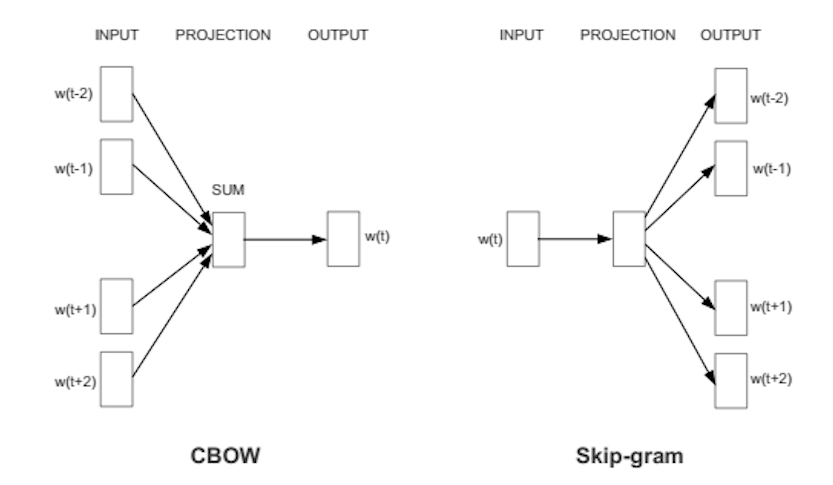
\includegraphics[width = 0.6\textwidth]{word2vec_skip_cbow.png}
	\caption[rnn_vanish]{Skip-gram和CBOW模型}
\end{figure}
Mikolov[??]2013提出了Word2Vec模型,解决了词向量训练速度慢,效率低的缺点。其利用了CBOW(Continuous Bag-of-words Model)和Skip-Gram的两种语言模型。其中CBOW的思想是利用词语的上下文词的信息来预测该单词。而Skip-Gram则采取一种和CBOW相反的策略,用中间的词的消息来预测上下文的词。

Mikolov创新性的提出了Hierarchical Softmax和负采样的词向量加速方法,为后续深度学习模型能在自然语言处理任务上打下了夯实的基础。对已经训练好的词向量,通过PCA等降维方法可在低纬度空间内实现可视化。

循环神经网络(Recurrent Neural Networks-RNN)已经在众多自然语言处理任务上取得了巨大成功。不同于传统过得前向反馈神经网络的同层节点无连接层于层之间节点有连接,循环神经网络引入了定向循环,可以处理序列数据。RNN中最大的缺陷是后面时间的节点对于前面节点的感知力下降,当网络深时训练效果下降。LSTM可以解决这一问题,目前LSTM是RNN中使用最广泛最成功的模型。

卷积神经网络不仅在图像处理上表现优异,在文本分类上同样表现不俗。kim[]提出的多卷积核文本分类CNN模型。模型第一层为预先训练好的词向量或者是随机初始化参数的词向量Embedding层,然后接一个宽度和词向量维数相同,长度通常为3、4、5的多个卷积核的卷积层,卷积层后是是较少参数的池化层,最大值池化层在分类的效果较好。池化层后的输出为文本提取出来的特征向量,最后连接一个全连接作为分类层。实验证明CNN在情感分析上能较好的性能。

\BiSection{文本立场分析相关技术}{Recommended figure format applied in \LaTeX}
文本立场分析与文本情感分析有着本质的区别,文本立场分析更加关注文本反应出作者对于某一特定目标主题所持的立场和倾向。立场分析需要结合目标主题和情感信息,这比单独考虑文本的消息更加具有有挑战,对模型的建模能力也有更高的要求。作为一项特殊的情感分析任务,立场分析问题主要是在给定了目标的前提下,判断这个文本的立场是“支持”或“反对”。作者在文本中评价的目标不一定是立场分析给定的目标,也可能立场分析给定的目标并没有直接出现在文本中。即使作者在文本中对目标/实体的态度是积极的,但推断出来的结果可能是作者对给定目标持反对的立场。

具有强大学习能力的基于特征的机器学习算法能够充分学习到文本的语法、语义等特征,因此受到了研究者的广泛关注。本节将介绍有监督的立场分析方法和若监督的立场分析方法。考虑到深度学习模型的立场分析研究逐渐增多且有成为主流的趋势,将在2.4小节单独介绍基于深度学习模型的立场分析研究状况。


\BiSubsection{基于有监督机器学习的文本立场分析技术}{2.3.1}

Anand等作为立场分析问题较早的研究者之一,抽取了网络论坛上4837篇分属14个不同话题的讨论,并针对此语料,构造了10种不同的特征。这10种特征包括一元/二元单词、文本长度、重复标点、线索词、句法依赖、语义依赖、广义依赖、上下文特征和LIWC(Liunguistics Inquiry Word Count)等。分别利用RIPPER和朴素贝叶斯两种算法验证了立场分析在不同特征集合下的效果。实验证明,应用了上下文特征可以有效提升实验效果,在不同子话题中同一分类模型表现有较大差异。对于Anand的研究,Hasan等研究者认为他们忽略了文本间意识形态和用户交互这两种对实验性能具有很大影响的约束。Hasan在研究中的文本序列模型是以相邻文本间的用户交互约束建立的,并利用了CRFs来解决序列标注问题。该研究为每位文本作者的意识形态以ILP建立基于话题领域、作者的意识形态约束模型。并且在实验中得到了比Anand正确率上2.9\%到10\%不等的提升。

社交文本以推特为例,具有长度较短且语言非正式等特点,Zhang针对这些特点提出了两部的学习系统。将社交媒体文本的三个立场“支持”、“反对”和“其他”转化为两次两分类的任务。第一步进行文本相关性检测,可以将无关文本作为“其他”类型检测出来;第二步使用立场倾向检测模型,对文本进行“支持”“反对”二分类。该研究在传统语言特征外还应用了LDA(Latent Dirichlet Allocation)生成的话题相关性、主题只是、情感词汇、词嵌入和表情符等多种不同的特征组合,为每一组子话题数据分别使用线性回归模型(Linear Regression,LR)建立立场分析模型。并且考虑到不同话题数据分布具有差异,对这各个子模型验证了不同超参数和特征集的组合方式。最后用实验证明了对不同子任务和子话题使用不同的特征组合的方式是有效的。

除了不同特征组合可以起到提升立场分类效果的作用,构建有差异的分类器组合也同样可以提升模型的立场分类效果和泛化能力。Xu等【】提出了选用该段落向量、浅层语义分析、LDA和其他语言学特征等,在线性SVMs、RBF核SVMs、Adaboost随机森林和随机森林等分类器中测试分类性能。并且该模型采用了对基分类器线性组合的方式提升模型表现,具体如公式~\ref{a23333}~所示。
\begin{equation}\label{a23333}
p(C|x)=\sum_{i=1}^m w_i \cdot p_i(C|x)
\end{equation}

式中$p_i(C|x)$为文本$x$在第$i$个分类器中被预测成立场类别$C$的概率;

$w_i$为线性模型中及分类器第$i$个基分类器的权重

$p(C|x)$为文本$x$在立场类别$C$中的概率

实验证明,该模型可以提高立场分类效果,并且可以直接被扩展到相似任务中。

\BiSubsection{基于弱监督机器学习的文本立场分析技术}{2.3.1}

弱监督学习是一种基于噪声训练数据的半监督学习方式。不同于以往基于可靠训练数据的有监督学习方式,弱监督学习基于的是不严密的假设生成训练数据。在训练数据中更可能含有错误和大量噪声。但该方法可以避免人工标注的高昂成本,且能在新语料、新话题中具有较好适用性。

Johnson等【】研究者提出了基于若干弱监督局部分类器的联合模型。每个局部分类器使用的训练语料为少量有立场和框架维度标注的种子集合,随后使用概率软逻辑框架组合各弱监督局部分类器。弱逻辑框架使用的训练数据是弱监督局部分类器的信息,之后利用合页-马尔科夫随机域 (hinge-loss Markov random fields,HL- MRFs)的图模型关系表示建立用于立场预测的规则。实验证明该模型能较准确的预测推特政治任务立场。

Ebrahimi【】提出了使用关系自扩展来实现弱监督学习的立场分类法扩展种子训练集。定义了三种立场相关约束:相似文本表达的立场相似、具有朋友关系的作者立场相似和文本作者对话题的立场相似。Ebrabimi为了匹配含噪音的少量标注集合,首先使用若干短语模式,然后利用基于统计关系学习的合页马尔科夫随机域模型标注文本立场,最后使用结合词典、多元词组和情感类型特征的线性和SVMs训练有监督的立场检测模型,并在SemEval数据集上表现良好。

Dias【】提出了使用启发式规则的方法自动标注Twitter文本,可以解决弱监督学习中语料标注的问题。该方法可以达到两重目的,既可以使用监督学习算法自动创建训练语料库开发预测模型,又可以补充预测立场检测模型。Dias构建了7条启发式规则构建训练语料,分析了六个不同的立场分析任务,取得了可观的成果,加权F值从52\%提升到了67\%。


\BiSection{基于深度学习的立场分析技术}{2.4}

近年来深度学习不仅在计算机视觉、语音识别等领域取得了卓越的成果,在自然语言处理中也有越来越多的研究者开始采用深度学习模型。不同于传统机器学习方法的手动特征工程,深度学习模型采用端到端的分类模式,能够自动抽取在参数学习中最优的特征表示。本节介绍深度学习模型在自然语言处理中的进展和立场分析方法上的应用。

Mikolov【】提出了一种基于循环神经网络的语言模型(Recurrent Neural Network Language Model, RNN-LM)。该网络具有三层结构,除了输入输出层还有上下文表示层,上下文表示层的信息拼接了上一时间和当前时间的两个信息,因此可以将全部历史信息保存在低纬度的向量空间中,大大增强了语言建模能力。实验表明,与已有的退避模型(Backoff Language Model)相比,使用多个 RNN-LM可以减少约50\%的困惑度(perplexity)。在“华尔街日报”任务上降低了18\%的错误率。Sundermeyer在【】为解决RNN-LM模型在反向误差传播函数时梯度消失/爆炸带来的巨大影响,采用了结合长短时记忆单元的循环神经网络(LSTM)该单元包含三个门:输入门、输出门和遗忘门,这样的结构可以解决梯度缩放问题且计算代价小。该模型在标准语料库上的困惑度指标比RNN-LM模型低8\%。

Zarrella等【】研究者同样使用了LSTM-RNN。并且用word2vec skip-gram方法训练了单词和短语的词向量。采集了218,179,858条Twitter文本,训练过程迭代100次,为文中出现的537,366个词汇和短语训得到256维的词向量。然后通过主题标签预测辅助任务来学习句子向量,然后被微调用于标记样本的立场检测。实验结果显示,该方法在5个话题文本立场检测任务中F值为0.678。

Yu【】提出了基于双向LSTM-RNN的模型,该模型包括词嵌入输入层、卷积层、长短时记忆单元层、双曲正切输入层和全连接分类层。卷积层的作用是提取多元词组的特征,长短时记忆单元的作用是学习潜在全局语义,池化层的额作用是减少参数并归纳句子表示。组合上述的知识表示用最后的双曲正切函数。实验证明此模型在中文立场分析任务中表现不错。

Wei【】为了解决在弱监督立场分析中标注数据缺失的问题,使用了两步框架。构建粗糙的二分类器,使用他们定义的softmax层在二分类训练数据中执行三分类任务。第一步利用有清晰倾向性的词汇和表情标注支持和反对两种立场,第二步将“支持”立场和“反对”立场概率差绝对值小于阈值的文本标注为第三类“中立”。以弱监督标注文本为基础,使用与有监督学习相似的深度学习模型得到的预测结果的方法被实验证明有效改善了训练数据在弱监督立场分析中缺失的问题。

近年来很多研究者开始关注在计算机视觉研究中较火的“注意力机制”并将其用于自然语言处理任务中。Bahdanau等【】第一次在机器翻译领域尝试“注意力机制”。该研究的编码器是双向RNN模型,解码器是gate-RNN模型。注意力机制被使用在解码器中用以发现编码器对当前翻译输出最有用的隐藏状态。注意力权重矩阵决定当前的翻译内容。除机器翻译之外,在语言模型和智能问答【】、图片描述文字生成【】、和句法树生成【】等领域也得到了广泛的应用。


\BiSection{本章小节}{2.5}


本章首先介绍了情感分析的常用技术和研究现状,然后从基于手工特征工程的机器学习方法和端到端的深度学习模型来年各个角度详细描述了立场分析检测的现有研究。基于特征筛选和分类器集成学习仍然是机器学习领域的主流,基于RNN/LSTM和CNNs等模型的工作是在深度学习领域上的主要方案。如何有效利用外部信息学习出更好的文本表示在现有的研究中仍然是一个重要的课题;其次,特有的预置话题包在分析任务任务中对最后的预测也起到了十分关键的作用,立场分析就有工作的重要方向就是如何将预置话题短语信息更好地利用上。